\documentclass[linenumbers]{aastex631}
\usepackage{graphicx}
\newcommand{\vdag}{(v)^\dagger}
\newcommand\aastex{AAS\TeX}
\newcommand\latex{La\TeX}

\begin{document}

\title{ASTR400B Research Proposal}

\author{Peter Hartman}
\affiliation{University of Arizona}

\begin{abstract}
    This project studies the evolution of the dark matter halo of the combined Milky Way-M31 merger remnant through the merger of the two galaxies. The affect of mergers on dark matter halos is key to understanding galaxy evolution, as most galaxies have undergone mergers in their histories. We focus on the mass and density profiles of the remnant and compare them to Hernquist profiles at several points throughout the merger process. This will give a description of the evolution of the halo through a merger. We find that for each of the 3 points considered in our analysis that the halo is well-fit by a Hernquist profile, with scale heights 97.95$\pm$0.18 $kpc$ at 4.286 $Gyr$, 89.8$\pm$0.16 $kpc$ at 6.429 $Gyr$, and 87.63$\pm$0.28 $kpc$ at 11.429 $Gyr$ from today. These findings indicate that the halo throughout the merger settles into a larger size than before, but retains the spherical profile it began with. These results provide insight on how the dark matter halos of merging galaxies react to each other and combine to create a new galaxy.
\end{abstract}

\keywords{Dark Matter Halos, Hernquist Profile, Merger Remnant, Major Merger, Spiral Galaxy}

\section{Introduction} \label{sec:intro}
Dark Matter Halos are the halos of invisible matter around the baryonic matter of galaxies that define them. Galaxies are defined by the presence of dark matter on top of the baryonic matter that makes up their structure, which is required to explain their rotation curves, and the halo is the structure of dark matter around the galaxy.

Dark matter halos are generally not spherical in shape, but they follow a spherical density profile that is described by a \cite{Hernquist} profile. The Hernquist profile is 
\begin{equation}
    \rho(r) = \frac{M}{2\pi} \frac{a}{r} \frac{1}{(r+a)^3} \label{eqn:Herndens}
\end{equation}
with M as the total halo mass, r as the distance from the center of mass of the galaxy, and a is the scale height, the distance to travel from the center where the density drops by a factor of $\frac{1}{e}$. This is a subset of spherical profiles, with the Navarro, Frenk, and White (1997), or NFW, profile, being another commonly used density profile. There are small differences between the two, but the spherical nature of the profiles are seemingly universal among observed galaxies.

We adopt a definition of "galaxy" \cite{Willman} defines as a gravitationally bound collection of stars whose properties cannot be explained a combination of baryons (i.e. "regular" matter: protons, electrons, neutrons, and what they form) and Newton's Law of Gravity. Hence they require some type of dark matter halo. The galaxies we study, the Milky Way and M31, are both spiral galaxies. They have a pattern of stars and dust that form into large arms that extend from the center of the galaxy.

Galaxy mergers are a common phenomenon throughout the Universe. They are the result of two galaxies colliding with each other and merging into a single galaxy. The \cite{Sotillo-Ramos} determined that most galaxies that are of comparable mass to the Milky Way have undergone mergers in their histories. Figure \ref{fig:mergers} shows us that mergers are quite common. While many galaxies have mergers, the ones that truly affect dark matter halos are major mergers, where the two galaxies have a mass ratio of 0.25 or higher, i.e. the more massive galaxy is at most 4 times more massive than the lower mass galaxy. As such, it is key to understand how these mergers to understand how galaxies change over time through galaxy evolution. Mergers leave behind a merger remnant, the newly-combined leftovers of the galaxy, which is a combination of the initial galaxy matter, with some lost through the merger process. These remnants are what we study in this work, specifically the Milky Way-M31 merger remnant.

\begin{figure}
    \centering
    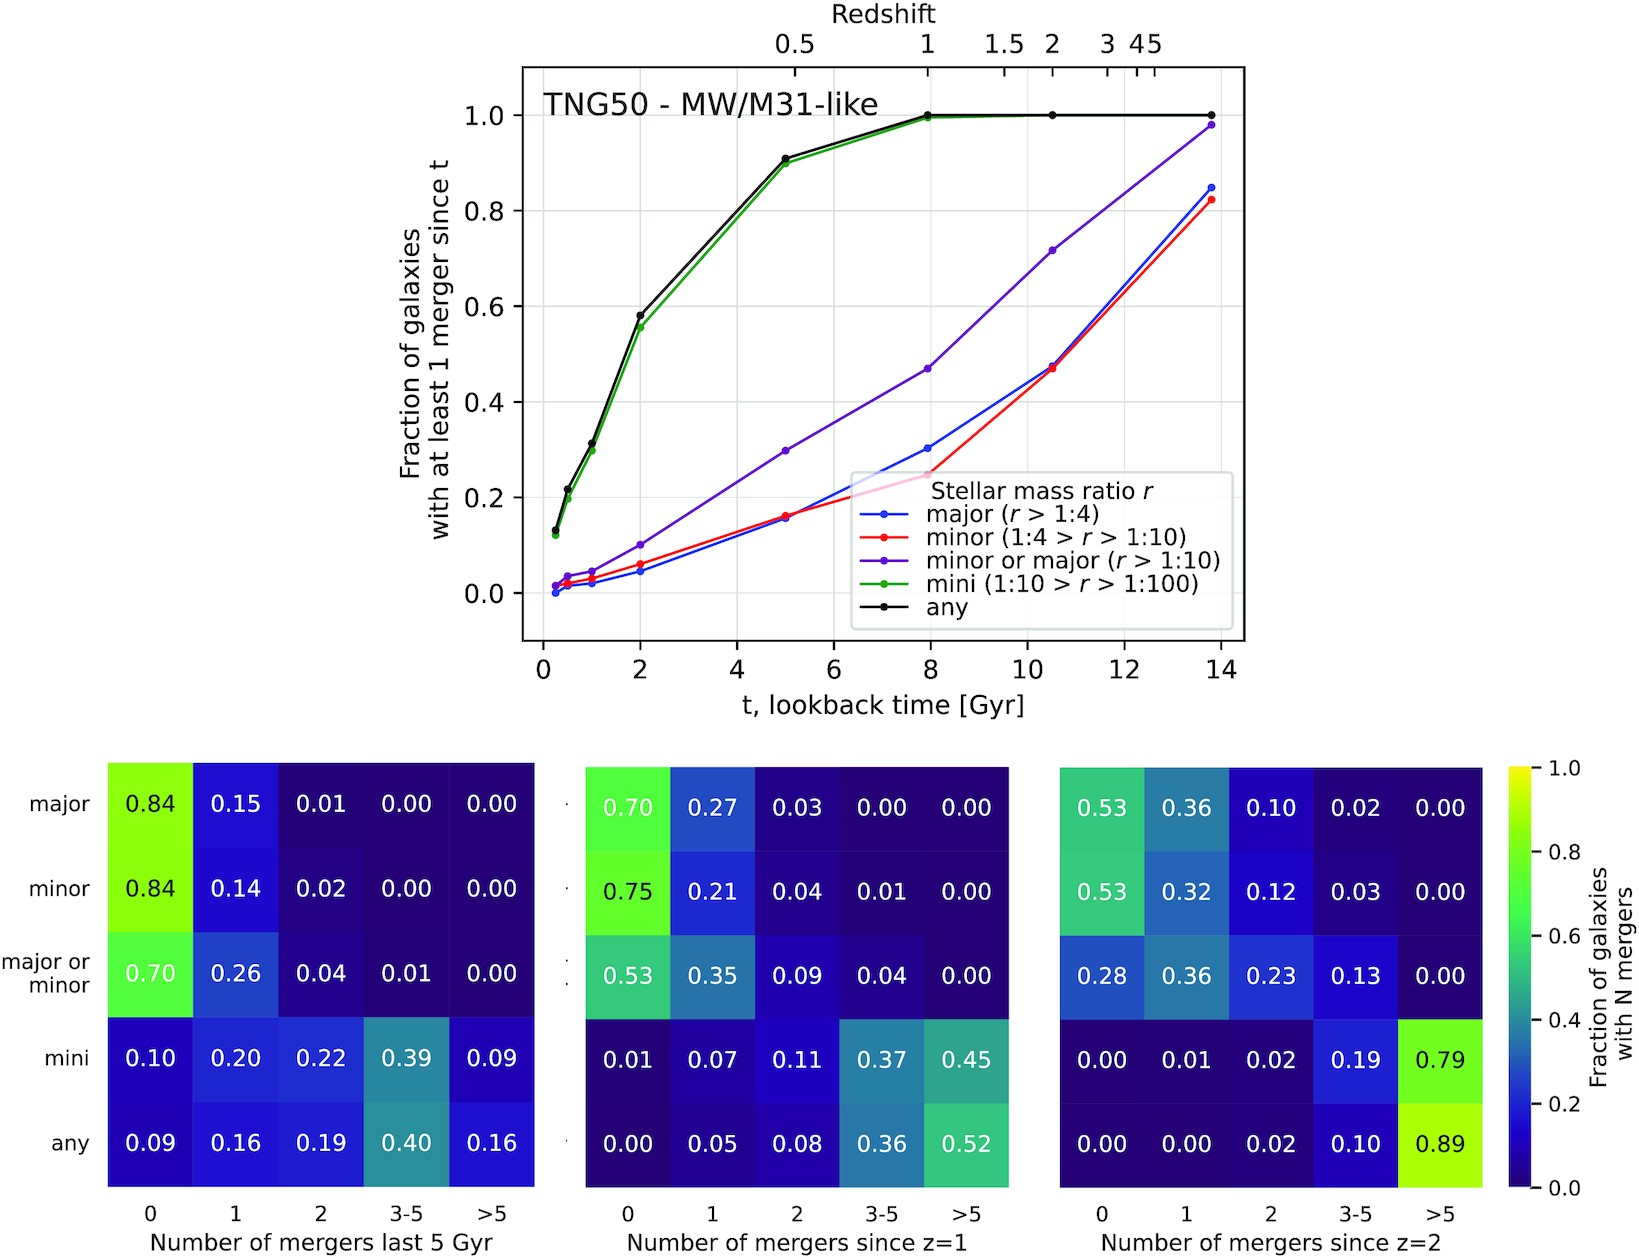
\includegraphics[width=\textwidth]{mergerNumbers.jpeg}
    \caption{The number of galaxies that have had mergers through time. (Top) The number of mergers through different times for Milky Way-like galaxies, and each line is for a different mass ratio. Note that almost every galaxy has undergone a merger since z=1, and 34\% have undergone a major merger since z=1. (Bottom) The fraction of galaxies having undergone a major merger at 3 specific time periods. The large number of mergers make it key to understand how mergers affect dark matter halos and thus, galaxy evolution. Figure from \cite{Sotillo-Ramos}.}
    \label{fig:mergers}
\end{figure}

Due to dark matter's purely gravitational interaction with baryons, its density profile is the most important component of dark matter's effect on galaxy evolution. The density profile of the halo is critical for the baryonic matter within the halo, as it determines the rotation rate of the galaxy and provides much of the mass to bind it. As such, the galactic structures we see heavily depend on the dark matter halo that they are embedded in.

While dark matter halos have a surprisingly universal spherically-averaged density profile, the triaxial nature of dark matter halos are important to consider. \cite{Meneghetti} determined that triaxial halos are necessary to match with CDM modeling, and the halo shape has an effect on stellar streams and nearby satellites due to the alteration of the potential. As such, there remains an open question in regards to the specific interactions of dark matter halos during mergers. Whether dark matter halos remain roughly spherical during their merger in terms of their density profiles is an important and open question.


\section{This Project}
This project is focused on the evolution of the dark matter halos of the Milky Way and M31 through their future collision and merger, and as the combined system settles. Specifically, we wish to determine how well-fit the dark matter halo profiles are to Hernquist profiles and how their extent changes throughout the merger and after the system settles.

We hope to answer how dark matter halo profiles evolve through mergers, which remains an open question. By understanding how dark matter halos evolve in galaxy mergers, we can work towards a better understanding of the structure of galaxies that have undergone mergers. The dark matter halo profile sets the gravitational potential of the galaxy, and thus sets much of the structural components of the galaxy. As such, studying the change in the halo structure will enable a better knowledge of how galaxies evolve through major mergers. Most large elliptical galaxies are thought to be the result of several major mergers, and the evolution of galaxies is intwined with their merger history.


\section{Methodology}
We are utilizing the simulations from \cite{sims}. These are N-body simulations where each particle is defined by its mass, position, and velocity, and their motions are found by considering gravitational forces from each other body and integrating their orbits over time. These simulations are important because they utilized current parallax and proper motion data to begin the simulations with proper kinematics. The simulations range from today to ~$11$ $Gyr$ in the future. The simulation considers the three galaxies M31, M33, and the Milky Way. The simulations assume Hernquist profiles for the dark matter halos of the constitutent galaxies, giving us a starting point for our studies.

We specifically focus on the positions of the dark matter halo particles. We collect data at 3 times in the process of the Milky Way-M31 merger: 4.3 $Gyr$, 6.4 $Gyr$, and 11.4 $Gyr$. At these times, the two galaxies are treated as part of the same system, so the particles are all collected into a single output file. These times correspond to just after the first collision event, while the system is beginning to finally merge, and after the system has settled. Each of these times have the dark matter particles in the combined system tracked and spherically averaged as shown in Figure \ref{fig:sph} to produce a mass and density profile, which are then fit to Hernquist profiles. The radii that are measured at are determined from the distance to the center of mass of the combined merger remnant.

The computations that will be completed are straightforward. The Hernquist fits are created using the \cite{Hernquist} profiles. The density profiles are shown in Equation \ref{eqn:Herndens} and the corresponding mass profiles are defined by
\begin{equation}
    M(r) = M\frac{r^2}{(r+a)^2}
\end{equation}

Where M is the total halo mass, r is the distance from the center of the spherical distribution, and a is the Hernquist scale height, the distance traveled such that the density falls by a factor of $\frac{1}{e}$. It is important to note that these distributions are purely radial, and thus are symmetric in $\phi$ and $\theta$. Once the data have been collected, the distribution is fit to a particular Hernquist profile, using the scale height as the fitting parameter. The fitting is done by the scipy package's curve fitting tool and is done via non-linear least-squares. The resulting scale height and 3$\sigma$ fitting errors are used to determine if the simulation profiles correspond to Hernquist profiles.

The plots in this paper are exactly what is described in words above: the simulation data profiles compared to theoretical profiles with best-fit scale heights. The resulting figures will aid in an understanding of the dark matter halo mass and density profile beyond the simple scale height fitting values because it will become more clear where the data diverges from theory or otherwise.

We expect that during the course of the merger, the Milky Way-M31 system will be no longer well-fit by a Hernquist profile as the two halos collide and the gravitational effects of the merger scatter the halo, leading to regions of over- and under-density. These regions would then settle over time and lead to the final state of the merger remnant returning to its initial Hernquist profile. This is motivated by the collisionless stars forming many tidal features and exhibiting non-uniform structure during mergers, and the dark matter particles are also collisionless particles that interact purely by gravity and should then exhibit similar behavior.

\begin{figure}
    \centering
    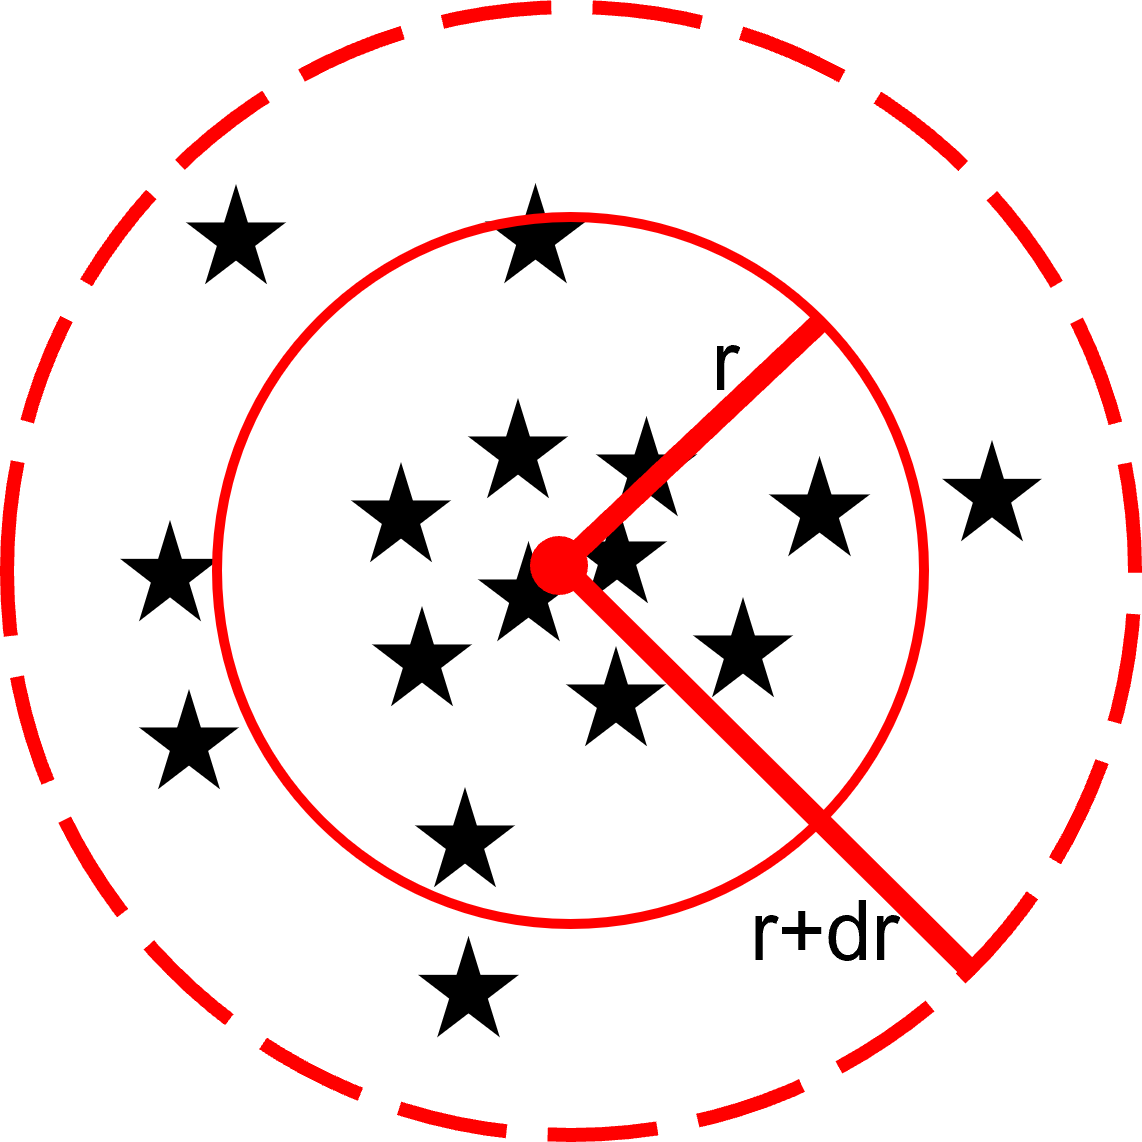
\includegraphics[width=7cm, height=7cm]{Spherical Averaging figure.png}
    \caption{A visual depiction of the process of spherical averaging to acquire a density profile. At each radius from the center of mass (shown as a red circle), shown by the solid red line, each star between the radius $r$ and the shell radius $r+dr$ is included in the total mass of the shell, which is divided by the volume of the shell to arrive at the density. The step $dr$ was chosen to be 0.1 $kpc$ for this paper. It is important to note that this star distribution is non-spherical, and the spherical averaging produces a spherical distribution.}
    \label{fig:sph}
\end{figure}

\section{Results}
The dark matter halo distribution for the combined Milky Way-M31 system 4.286 $Gyr$ from today is shown in \ref{fig:300}. This result features a very strong fit to a Hernquist profile with scale height 97.95 and 3$\sigma$ error of 0.18 $kpc$. All errors are given as 3$\sigma$ errors. The density profile has more scatter, but fits to a Hernquist profile in a similar way. The small errors at 3$\sigma$ provide strong confidence in the presence of a Hernquist halo. This time is mid-merger, so this result tells us that Hernquist profile halos tend to remain Hernquist throughout their merger events.

The halo distribution 6.429 $Gyr$ from today is shown in \ref{fig:450}. This result keeps up the tight fit to Hernquist profiles as the merger event winds down. The combined Milky Way-M31 dark matter halo fits to a Hernquist profile with scale height 89.8$\pm$0.16 $kpc$. This time shows us a decrease in scale height, but not a change from a Hernquist profile, telling us that the merger remnant has begun to coalesce into its final profile.

The halo distribution 11.429 $Gyr$ from today is shown in \ref{fig:800}. This result is again a tight Hernquist fit, with a scale height of 87.63$\pm$0.28 $kpc$. This is the final state of the merger remnant, after it has settled. The scale height decrease indicates this to us, and the Hernquist fit tells us that halos tend to settle into these spherical profiles over time after mergers.

\begin{figure}
    \centering
    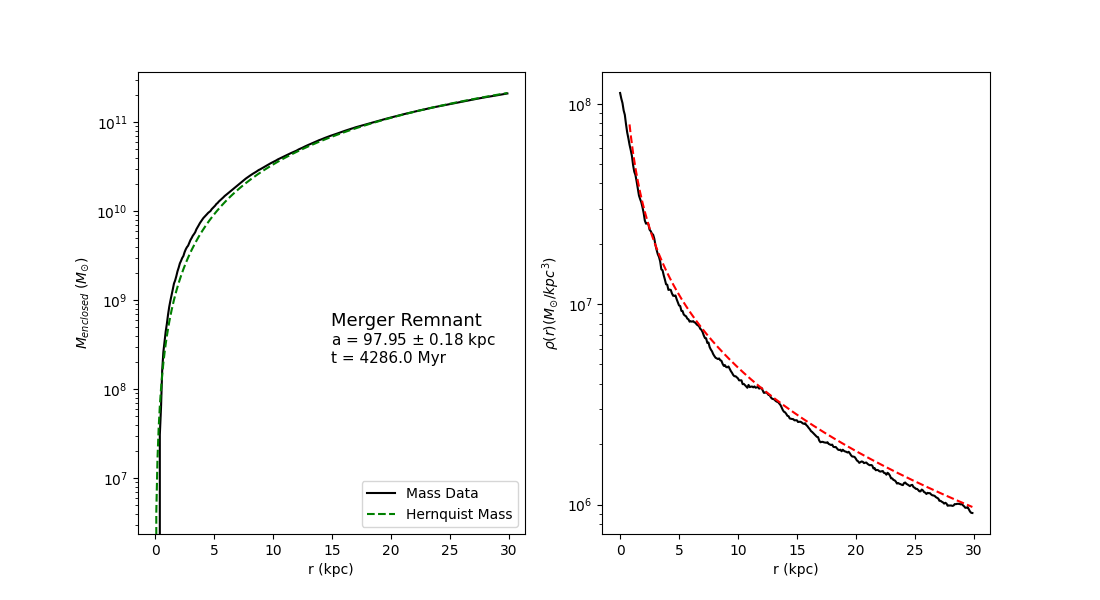
\includegraphics[width=\textwidth]{Snap300FitswithConcat.png}
    \caption{(Left) The mass profile of the combined Milky Way-M31 system is plotted as a black solid line and the best-fit Hernquist mass profile is plotted as a green dashed line. The best-fit scale height is given in $kpc$ as well as the time that the halo is seen at. This point in time is near the start of the merger, as the first collision event is finishing and the galaxies are coming close for another collision. The distance from the center of mass of the combined system is shown on the x-axis, and the total mass enclosed within a sphere of the associated radius is shown on the y-axis. (Right) The density of stars in a spherical shell with thickness 1 $kpc$ at the associated radius is shown on the y-axis, and the Hernquist density profile that is associated with the scale height shown in the left panel is plotted as a red dashed line. Notably, the data are exceptionally well-fit by a Hernquist profile, even just after the merger at this time.}
    \label{fig:300}
\end{figure}

\begin{figure}
    \centering
    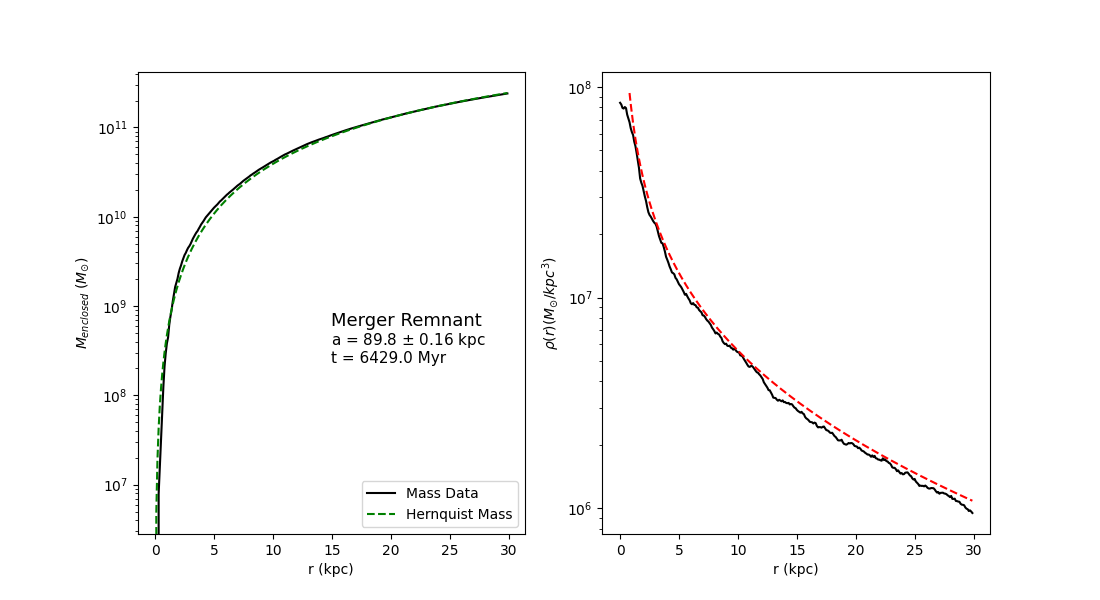
\includegraphics[width=\textwidth]{Snap450withConcat.png}
    \caption{(Left) the mass of the combined Milky Way-M31 system is plotted as a black solid line and the best-fit Hernquist mass profile is plotted as a green dashed line. The best-fit scale height is given in $kpc$ as well as the time that the halo is seen at. This point is time is as the merger is beginning to settle after the first collision events. The distance from the center of mass of the combined system is shown on the x-axis, and the total mass enclosed within a sphere of the associated radius is shown on the y-axis. (Right) The density of stars in a spherical shell with thickness 1 $kpc$ at the associated radius is shown on the y-axis, and the Hernquist density profile that is associated with the scale height shown in the left panel is plotted as a red dashed line. This point in time features a smaller scale height than previous points in time, indicating that the halo is settling.}
    \label{fig:450}
\end{figure}

\begin{figure}
    \centering
    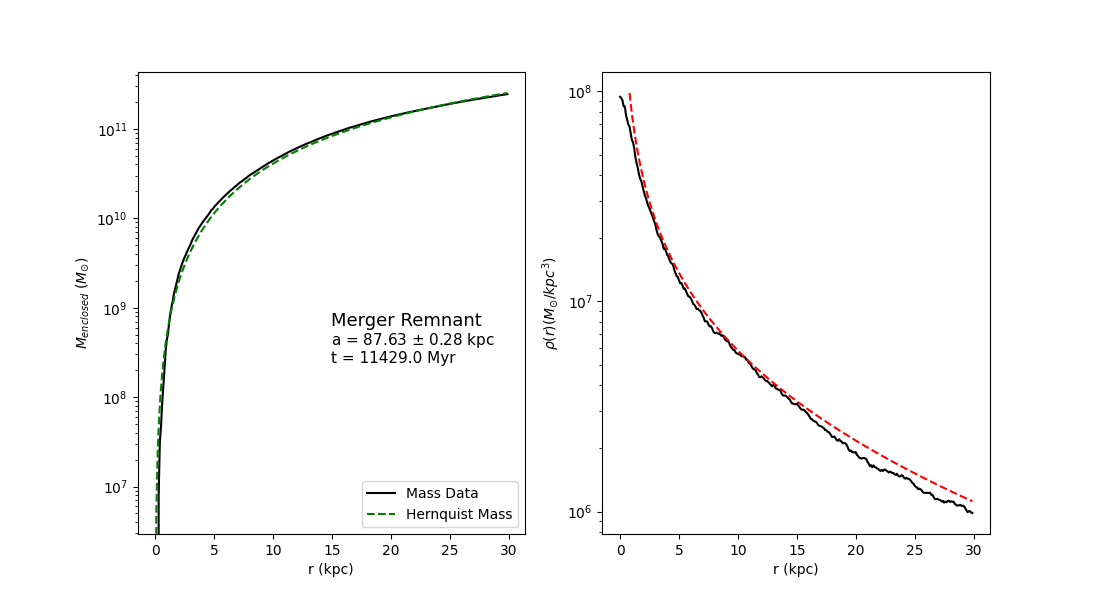
\includegraphics[width=\textwidth]{Snap800Fits.png}
    \caption{(Left) the mass of the combined Milky Way-M31 system is plotted as a black solid line and the best-fit Hernquist mass profile is plotted as a green dashed line. The best-fit scale height is given in $kpc$ as well as the time that the halo is seen at. This point is time is at the end of the merger, as the combined merger remnant has settled. The distance from the center of mass of the combined system is shown on the x-axis, and the total mass enclosed within a sphere of the associated radius is shown on the y-axis. (Right) The density of stars in a spherical shell with thickness 1 $kpc$ at the associated radius is shown on the y-axis, and the Hernquist density profile that is associated with the scale height shown in the left panel is plotted as a red dashed line. This point in the simulation features a smaller scale height than previous times, and has a strong fit to a Hernquist profile, both results that were expected.}
    \label{fig:800}
\end{figure}

\section{Discussion}
We find that during the start of the merger, shown in Figure \ref{fig:300}, the mass and density profiles of the galaxies in simulation are well-fit by a Hernquist profile. This is quite different than our expectation that the halo would be disrupted. Previous work by \cite{Despali} has shown that halos become triaxial after mergers and smooth out over time, but it appears that the triaxial shape does not affect the spherically averaged profile. This is indicative that the dark matter halo of a galaxy is not greatly affected by 
mergers.

When looking at the other times, we see similar profiles. In Figure \ref{fig:450}, we again see a strong fit to a Hernquist profile, and the lower scale height indicates the settling of the system that we expect, but the strength of the fit is again counter to what was expected. This tells us how galaxies settle through mergers, an important part of their evolution.

At the late time shown in Figure \ref{fig:800}, we also see a strong Hernquist fit and an even lower scale height. This fits with our expectations for after the system settles. The scale height, while lower than before, is significantly higher than the current scale heights of the Milky Way and M31 halos, which are both ~60 $kpc$. This increase is expected from the merger creating more scatter in the velocities of the stars from the addition of the two kinematics.

There are potential issues with the above analysis, though. The method to measure the halos was a spherical average, where each particle within a specific radius range was used. This leads to a loss in spatial accuracy, as even for different halo shapes we recover a spherical distribution by definition. While there may be extreme cases in which the profile is not a Hernquist profile, it is very likely that we recover a Hernquist profile for the dark matter that is very dense near the center of the merger, so our results are biased towards a purely spherical shape.

\section{Conclusions}
Dark matter halos are key parts of defining galactic structure, and their tendency to change in the process of galaxy mergers means that they need to be studied throughout the merger process. The halo begins from a spherical density distribution described by a Hernquist profile, but how the halo changes is an important question. The halo is key because it sets the gravitational potential of the galaxy, defining the region where baryons can form luminous parts of galactic structure.

We find that the dark matter halo remains well-fit to a spherical Hernquist profile and has a scale height that decreases with time. This indicates that the dark matter halos do not change their broad structure in terms of mass during the merger, simply growing larger during the merger and settling into a more compact spherical distribution over time. This is opposed to the original hypothesis, which anticipated that the halo would move out of a spherical Hernquist profile and then return to it after given time to settle.

This work could be improved by considering more different times, and computing the scale heights for each time in the simulation, instead of choosing 3. The process of spherical averaging could be improved by determining the proper step to take beyond the initial radius when computing the density to include as few stars as possible while remaining descriptive, instead of simply choosing one arbitrarily. The radius to compute the mass profile out to could also be better found by computing the virial radius of the dark matter halo and going to that instead of choosing 100 $kpc$.

\section{Acknowledgements}
This research made use of Astropy, a community-developed core Python package for Astronomy \citep{2018AJ....156..123A, 2013A&A...558A..33A}, matplotlib, a Python library for publication quality graphics \citep{Hunter:2007}, NumPy \citep{2011CSE....13b..22V}, SciPy (Jones et al. (2001–),Open source scientific tools for Python. http://www.scipy.org/), and the IPython package \citep{2007CSE.....9c..21P}. Dr. Gurtina Besla and Mr. Hayden Foote both provided immense assistance throughout this project, from determining the topic to writing this report.
\bibliography{sample631}

\end{document}